\section{Design}
\subsection{UI Design}
Bevor mit der Entwicklung des Frontends begonnen werden kann, muss geplant werden, wie dieses aussehen soll. Um ein möglichst gutes Ergebnis zu erzielen, ist es wichtig sich folgende Fragen zu stellen \footcite{ui_design_questions}:

\begin{itemize}
	\item Welche Anforderungen werden an die Webseite gestellt?
	\item Welche Benutzergruppen werden die Applikation verwenden?
	\item Was sind die Bedürfnisse der einzelnen Gruppen?
\end{itemize}

Durch das Beantworten der einzelnen Fragen, kann schnell herausgefunden werden, welche Anforderungen an das Frontend gestellt werden. Da der Aufgaben-Coach von komplett verschiedenen Benutzergruppen verwendet und damit gearbeitet wird, sollte das UI mögichst simpel und effizient gestaltet werden. Folgende Anforderungen konnten herauskristallisiert werden:

\begin{itemize}
	\item Usability \\
		Bei einer der Benutzergruppen handelt es sich um Schüler. Die Gruppe Schüler ist die Hauptnutzergruppe der Applikation und soll desshalb besonders gut abgeholt werden. \\
		
\begin{minipage}{\textwidth}
	\begin{figure}[H]
	\centering
		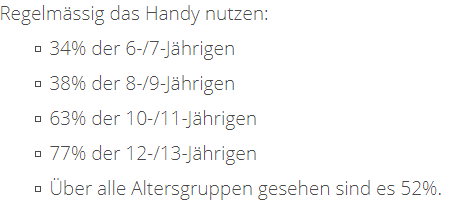
\includegraphics[width=8cm, keepaspectratio]{images/HandyNutzung.png}
		\caption{Handynutzung Primarschüler}
	\end{figure}
\end{minipage}
		
		Wie der Abbildung oben entnommen werden kann, verwenden etwa 52\% der Primarschüler der Schweiz regelmässig ein Handy \footcite{smartphone_usage}. Bei den Sekundarschülern ist diese Zahl sogar noch höher. Um also möglichst gut auf die Bedürfnisse der Schüler einzugehen, soll der komplette, für sie gedachte, Teil, ebenfalls über Tablets und Mobiles bedienbar sein.
		
	\item Struktur \\
		Internetnutzer haben in der Regel eine relativ kurze Aufmerksamkeisspanne. In den letzten 15 bis 20 Jahren ist diese um etwa 30\% zurückgegangen. Das bedeutet, dass man als Designer einer Webapplikation immer weniger Zeit hat, beim Benutzer einen positiven ersten Eindruck zu hinterlassen und ihm die Information zu liefern, weswegen er die Webseite besucht \footcite{attention_span}. \\ 
		Das Wohlbefinden des Benutzers darf auf keinen Fall vernachlässigt werden, denn ein positives Erlebnis wirkt sich direkt auf die Zeit aus, die er auf der Webseite verbringt und ob er sie erneut besucht \footcite{positiv_experience}.
		Aus diesem Grund soll anhand der Strukur auf den ersten Blick klar sein, was möglich ist und was nicht.
		
	\item Navigation \\
		Die Navigation über die Webseite soll so einfach und simpel wie möglich gehalten werden. Es soll möglich sein von jedem beliebigen Punkt der Webseite in kürzester Zeit zu einem beliebig anderen Punkt navigieren zu können.
	
	\item Orientierung \\
		Die Benutzer der Applikation sollen sich auf der Webseite zurecht finden und zu jedem Zeitpunkt wissen, wo sie sich befinden. Eine einfache Orientierung ist der Grundstein für das Wohlbefinden der Benutzer und soll deshalb berücksichtigt werden.
		
	\item Kontrast \\
		Die dargestellten Elemente sollen gut erkennbar sein und nicht in der Webseite versinken. Natürlich soll damit nicht übertrieben und mit knalligen Farben um sich geworfen werden.
\end{itemize}

Basierend auf den oben aufgelisteten UI-Design Anforderungen, wurden folgende Entscheidungen getroffen:

\begin{itemize}
	\item Usability \\
		Webseiten welche über Tablets und Mobilies verwendet werden, sollten niemals überladen sein. Aus diesem Grund sollen die Teile der Applikation, welche für die Schüler gedacht sind, schlicht und einfach gehalten werden. Wo auch immer möglich soll auf lange Texte verzichtet werden \footcite{usability}. Die einzelnen Seiten der Webapplikation sollen nur die für sie gedachte Aufgabe lösen.
		
	\item Struktur \\
		Um eine möglichst benutzerfreundliche Struktur aufzubauen, soll auf ein Kompromiss zwischen, ''eine Webseite so einfach wie möglich halten und nur eine bestimmte Aufgabe lösen zu lassen'' und ''eine bestimmte Aufgabe mit so wenigen Klicks wie möglich lösen zu können'', gesetzt werden. \\
		
	\item Navigation \\
		Um eine schnelle Navigation zu ermöglichen, soll die Applikation in fünf Bereiche aufgeteilt werden, welche über die Navigationsleite erreichbar sind. Dabei soll es sich um folgende Bereiche handeln: Statistiken, Klassenverwaltung, Adminpanel, Schulstoff und User. 
		
	\item Orientierung \\
		Um den Benutzern eine möglichst gute Orientierung zu gewähren, sollen Breadcrumbs eingebaut werden. Um zusätzlich eine einheitliche Navigation durch die Applikation zu bieten, sollen die Breadcrumbs auch zum navigieren verwendet werden können.
		
	\item Kontrast \\
		Es soll auf knallige Farben und Eye­cat­cher verzichtet werden. Wichtige Elemente sollen zwar mit Farbe hervorgehoben werden, jedoch nicht dadurch auffallen. Die schlichte Gestalltung der Webseite soll die Aufmerksamkeit auf die entsprechenden Elemente leiten.
\end{itemize}


\subsection{Mockup}
Anhand der getroffenen Entscheidungen wurden Mockups erstellt. Der Entscheid zum Erstellen von Mockups hat mehrere Gründe und bietet auch gleich verschiedene Vorteile. Während dem Erstellen von Mockups kann bereits früh erkannt werden, ob wichtige Punkte vergessen oder vernachlässigt wurden. Sobald die Mockups fertiggestellt sind, können damit bereits erste Tests durchgeführt werden. Zum Beispiel kann geprüft werden, ob alle geforderten funktionalen Anforderungen erfüllt werden und es können erstmals Usability-Tests durchgeführt werden, was viel Zeit und unnötige Arbeit ersparen kann \footcite{mockups}. \\

Nachfolgend werden einige Beispiele für Ergebnisse der getroffenen Entscheidungen für die Mockups aufgelistet. Im Anhang sind alle gemachten Mockups zu finden. \\ %TODO Link zu Anhang einbauen. und Mockups anhängen

Usability: \\
Auf dem Dashboard wird der Wochenplan des Schülers, gefolgt von den derzeit besuchten Fächern, knapp und ersichtlich aufgelistet. \\
\begin{minipage}{\textwidth}
	\begin{figure}[H]
	\centering
		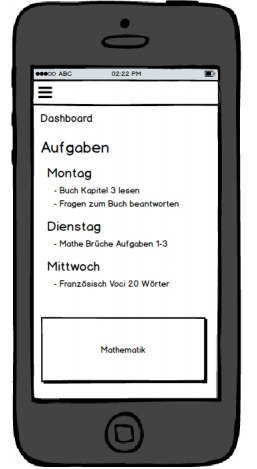
\includegraphics[width=5cm, keepaspectratio]{images/Mockups/Dashboard_Smartphone.png}
		\caption{Mockup Smartphone Dashboard}
	\end{figure}
\end{minipage}


Struktur: \\
Die Aufgabe dieser Seite ist es, neue Fragen zu definieren. Mit dem Risiko die Seite ein wenig zu überladen, dem Benutzer jedoch eine bessere Übersicht zu bieten, wurde ein Kompromiss eingegangen und entschieden, dass auch die dazugehörenden Hilfestellungen erfasst werden können. \\
\begin{minipage}{\textwidth}
	\begin{figure}[H]
	\centering
		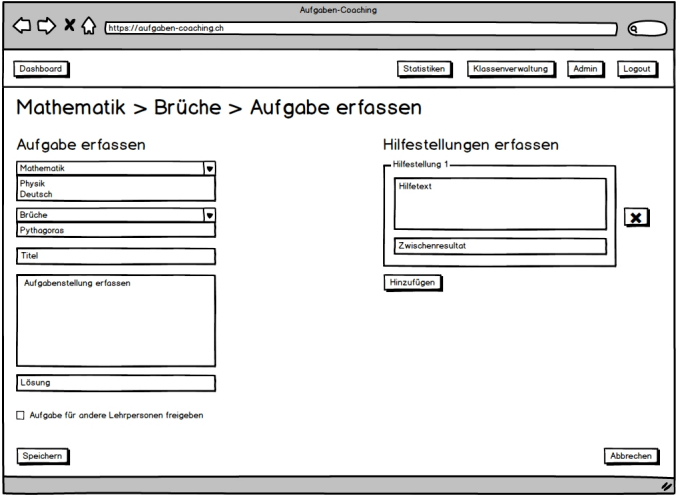
\includegraphics[width=\textwidth, keepaspectratio]{images/Mockups/AufgabeErfassen_Desktop.png}
		\caption{Mockup Aufgabe erfassen Desktop}
	\end{figure}
\end{minipage}


Navigation: \\
In der Navigationsbar sind die fünf definierten Bereiche ersichtlich. Dashboard stellt den Schulstoff Bereich dar, Statistiken die Statistiken, Klassenverwaltung die Klassenverwaltung, Admin das Adminpanel und Logout/Login die User. \\
\begin{minipage}{\textwidth}
	\begin{figure}[H]
	\centering
		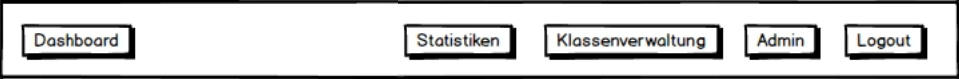
\includegraphics[width=\textwidth, keepaspectratio]{images/Mockups/Navigationsleiste_Desktop.png}
		\caption{Mockup Navigationsbar Desktop}
	\end{figure}
\end{minipage}


Orientierung: \\
Durch die Breadcrumbs wird hierarchisch dargestellt, wo man sich aktuell in der Webapplikation befindet. Mit einem Klick auf die übergeordneten Bereiche, navigiert man sofort an die gewünschte Stelle. \\
\begin{minipage}{\textwidth}
	\begin{figure}[H]
	\centering
		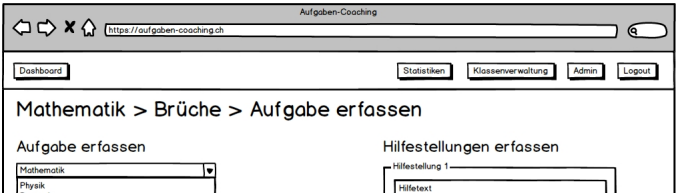
\includegraphics[width=\textwidth, keepaspectratio]{images/Mockups/Breadcrumbs_Desktop.png}
		\caption{Mockup Breadcrumbs Desktop}
	\end{figure}
\end{minipage}


Kontrast: \\
Da die Mockups in schwarz und weiss erstellt wurden, gibt es hierfür kein Beispiel. Die Entscheidung wurde natürlich dennoch in die Entwicklung miteinbezogen.



\subsection{Effektive Webseite}

\newpage